% Options for packages loaded elsewhere
\PassOptionsToPackage{unicode}{hyperref}
\PassOptionsToPackage{hyphens}{url}
%
\documentclass[
]{book}
\usepackage{amsmath,amssymb}
\usepackage{lmodern}
\usepackage{iftex}
\ifPDFTeX
  \usepackage[T1]{fontenc}
  \usepackage[utf8]{inputenc}
  \usepackage{textcomp} % provide euro and other symbols
\else % if luatex or xetex
  \usepackage{unicode-math}
  \defaultfontfeatures{Scale=MatchLowercase}
  \defaultfontfeatures[\rmfamily]{Ligatures=TeX,Scale=1}
\fi
% Use upquote if available, for straight quotes in verbatim environments
\IfFileExists{upquote.sty}{\usepackage{upquote}}{}
\IfFileExists{microtype.sty}{% use microtype if available
  \usepackage[]{microtype}
  \UseMicrotypeSet[protrusion]{basicmath} % disable protrusion for tt fonts
}{}
\makeatletter
\@ifundefined{KOMAClassName}{% if non-KOMA class
  \IfFileExists{parskip.sty}{%
    \usepackage{parskip}
  }{% else
    \setlength{\parindent}{0pt}
    \setlength{\parskip}{6pt plus 2pt minus 1pt}}
}{% if KOMA class
  \KOMAoptions{parskip=half}}
\makeatother
\usepackage{xcolor}
\IfFileExists{xurl.sty}{\usepackage{xurl}}{} % add URL line breaks if available
\IfFileExists{bookmark.sty}{\usepackage{bookmark}}{\usepackage{hyperref}}
\hypersetup{
  pdftitle={Big Book of DRIVES Notes},
  pdfauthor={Matthew Schuelke},
  hidelinks,
  pdfcreator={LaTeX via pandoc}}
\urlstyle{same} % disable monospaced font for URLs
\usepackage{longtable,booktabs,array}
\usepackage{calc} % for calculating minipage widths
% Correct order of tables after \paragraph or \subparagraph
\usepackage{etoolbox}
\makeatletter
\patchcmd\longtable{\par}{\if@noskipsec\mbox{}\fi\par}{}{}
\makeatother
% Allow footnotes in longtable head/foot
\IfFileExists{footnotehyper.sty}{\usepackage{footnotehyper}}{\usepackage{footnote}}
\makesavenoteenv{longtable}
\usepackage{graphicx}
\makeatletter
\def\maxwidth{\ifdim\Gin@nat@width>\linewidth\linewidth\else\Gin@nat@width\fi}
\def\maxheight{\ifdim\Gin@nat@height>\textheight\textheight\else\Gin@nat@height\fi}
\makeatother
% Scale images if necessary, so that they will not overflow the page
% margins by default, and it is still possible to overwrite the defaults
% using explicit options in \includegraphics[width, height, ...]{}
\setkeys{Gin}{width=\maxwidth,height=\maxheight,keepaspectratio}
% Set default figure placement to htbp
\makeatletter
\def\fps@figure{htbp}
\makeatother
\setlength{\emergencystretch}{3em} % prevent overfull lines
\providecommand{\tightlist}{%
  \setlength{\itemsep}{0pt}\setlength{\parskip}{0pt}}
\setcounter{secnumdepth}{5}
\usepackage{booktabs}
\usepackage{booktabs}
\usepackage{longtable}
\usepackage{array}
\usepackage{multirow}
\usepackage{wrapfig}
\usepackage{float}
\usepackage{colortbl}
\usepackage{pdflscape}
\usepackage{tabu}
\usepackage{threeparttable}
\usepackage{threeparttablex}
\usepackage[normalem]{ulem}
\usepackage{makecell}
\usepackage{xcolor}
\ifLuaTeX
  \usepackage{selnolig}  % disable illegal ligatures
\fi
\usepackage[]{natbib}
\bibliographystyle{apalike}

\title{Big Book of DRIVES Notes}
\author{Matthew Schuelke}
\date{2022-05-25}

\begin{document}
\maketitle

{
\setcounter{tocdepth}{1}
\tableofcontents
}
\hypertarget{about}{%
\chapter{About}\label{about}}

This is a place to store and share documentation about the \href{https://roelab.wustl.edu}{DRIVES Lab} as \href{https://wustl.edu/}{Washington University}.

\hypertarget{personnel}{%
\chapter{Personnel}\label{personnel}}

\begin{table}
\centering\begingroup\fontsize{9}{11}\selectfont

\begin{tabular}{l|l|l|l|l|r|l|l}
\hline
Category & Title & Last Name & First Name & Email & Telephone & Position & Department\\
\hline
current & Dr. & Babulal & Ganesh & babulalg@wustl.edu & 3142862435 & Asst Prof of Neurology & Neurology - Administration\\
\hline
current &  & Bayat & Sayeh & sayeh.bayat@mail.utoronto.ca &  &  & \\
\hline
current &  & Doherty & Jason & djason@wustl.edu & 3142862435 & Sr Statistical Data Analyst & Neurology - Administration\\
\hline
current & Ms. & Johnson & Ann & ajohnson22@wustl.edu & 3143620881 & Clinical Research Coord II & CCS - Recharge Centers\\
\hline
current & Miss. & Walker & Alexis & alexis.walker@wustl.edu & 3147471474 & Clinical Research Coordinator I & Neurology - Administration\\
\hline
current &  & Pina & Yasmin & pina@wustl.edu & 3142732279 & Clinical Research Coordinator I & Neurology - Administration\\
\hline
current &  & Murphy & Samantha & msamantha@wustl.edu & 3142862435 & Senior Clinical Research Coordinator & Neurology - Administration\\
\hline
current & Dr. & Roe & Catherine & cathyr@wustl.edu & 3142862435 & Assoc Prof of Neurology & Neurology - Administration\\
\hline
current &  & Williams & Monique & monique.williams4@bjc.org &  &  & \\
\hline
current & Dr. & Schuelke & Matthew & schuelke@wustl.edu & 3143620000 & Medical Informaticist III & Biostatistics\\
\hline
current &  & Wisch & Julie & julie.wisch@wustl.edu & 3147478423 & Sr Neuroimaging Engineer & Neurology - Administration\\
\hline
current & Dr. & Chen & Ling & lingchen@wustl.edu & 3147472373 & Asst Prof of Biostatistics & Biostatistics\\
\hline
collaborators & Dr. & Ances & Beau & bances@wustl.edu & 3147478423 & D J Brennan Prof of Neurology & Neurology - Administration\\
\hline
collaborators & Dr. & Benzinger & Tammie & benzingert@wustl.edu & 3143625950 & Prof of Radiology & Radiology - Main - Clinical - Diagnostic - Neuroradiology\\
\hline
collaborators & Dr. & Niven & Anne & fagana@wustl.edu & 3143623453 & Prof of Neurology & Neurology - Administration\\
\hline
collaborators & Dr. & Head & Denise & dhead@wustl.edu & 3149358732 & Professor of Psychological and Brain Sciences & A\&S - Psychological \& Brain Sciences\\
\hline
\end{tabular}
\endgroup{}
\end{table}

\hypertarget{infrastructure}{%
\chapter{Infrastructure}\label{infrastructure}}

\begin{figure}
\centering
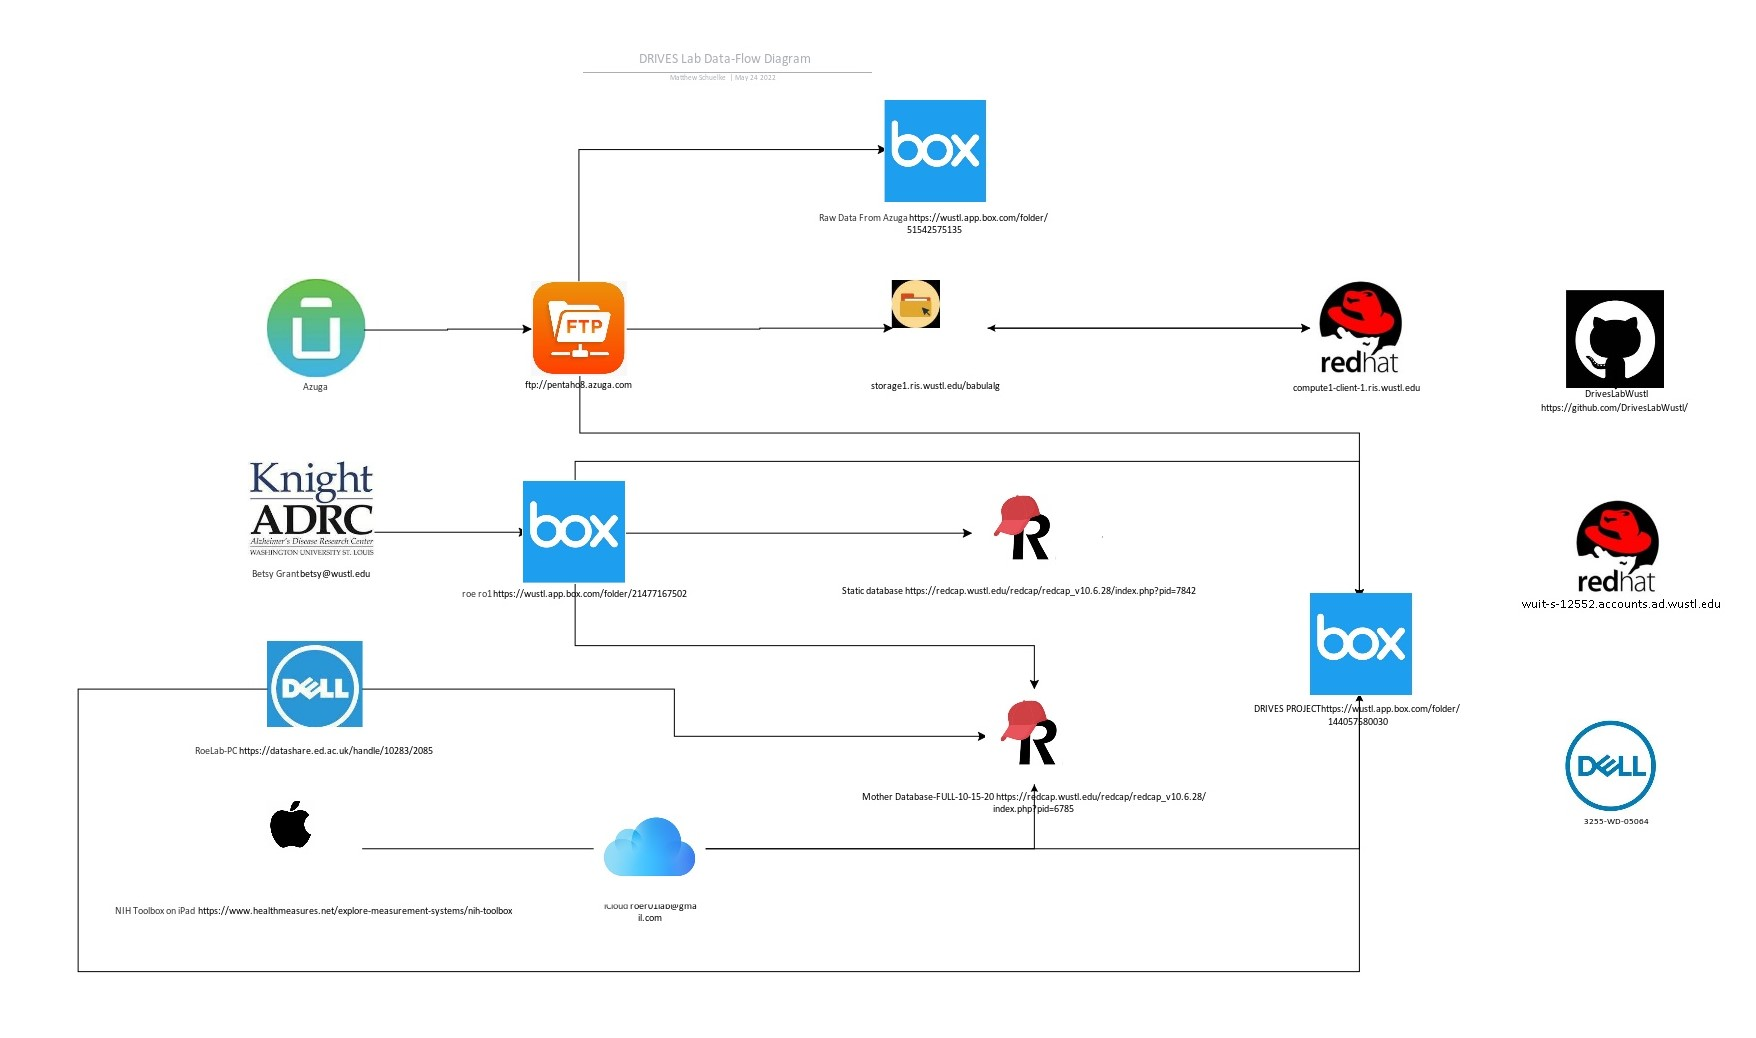
\includegraphics[width=1\textwidth,height=\textheight]{img/Data-Flow Diagram.jpg}
\caption{Data-Flow Diagram}
\end{figure}

The \href{img/Data-Flow\%20Diagram.vsdx}{Data-Flow Diagram.vsdx} can be edited for free at \href{https://products.aspose.app/diagram/editor}{aspose.app}.

\hypertarget{sources}{%
\section{Sources}\label{sources}}

\hypertarget{azuga}{%
\subsection{Azuga}\label{azuga}}

Driving data is collected from study participants via an \href{https://www.azuga.com/}{Azuga} GPS device plugged into their vehicle's \href{https://en.wikipedia.org/wiki/On-board_diagnostics}{OBD} port.

Azuga pushes files daily to their \href{ftp://pentaho8.azuga.com}{ftp server}.

This server can be accessed via plain FTP (insecure). Credentials are available in the credential store.

\hypertarget{knight-adrc}{%
\subsection{Knight ADRC}\label{knight-adrc}}

The \href{https://knightadrc.wustl.edu/}{Charles F. and Joanne Knight Alzheimer Disease Research Center (Knight ADRC)} supports researchers and the surrounding community in the pursuit of answers that will lead to improved diagnosis and care for persons with Alzheimer disease (AD). The Center is committed to the long-term goal of finding a way to effectively treat and prevent AD.

Our contact in \href{mailto:betsy@wustl.edu}{Betsy Grant}.

\hypertarget{lab-ipad}{%
\subsection{Lab iPad}\label{lab-ipad}}

The iPad is used to administer select measures from the \href{https://www.healthmeasures.net/explore-measurement-systems/nih-toolbox}{NIH Toolbox}.

\hypertarget{roelab-pc}{%
\subsection{RoeLab-PC}\label{roelab-pc}}

The RoeLab-PC is used to collect \href{https://datashare.ed.ac.uk/handle/10283/2085}{Deary-Liewald Reaction time} data.

\hypertarget{storage}{%
\section{Storage}\label{storage}}

\hypertarget{icloud}{%
\subsection{iCloud}\label{icloud}}

The lab iPad is backed up to iCloud.

\hypertarget{box-folder---roe-ro1}{%
\subsection{Box Folder - roe ro1}\label{box-folder---roe-ro1}}

Betsy shares ADRC files \href{https://wustl.app.box.com/folder/21477167502}{here}.

\hypertarget{box-folder---raw-data-from-azuga}{%
\subsection{Box Folder - Raw Data from Azuga}\label{box-folder---raw-data-from-azuga}}

A script monitors the Azuga ftp server and copies the files \href{https://wustl.app.box.com/folder/51542575135}{here}.

\hypertarget{box-folder---drives-project}{%
\subsection{Box Folder - DRIVES PROJECT}\label{box-folder---drives-project}}

Various scripts and programs backup all data \href{https://wustl.app.box.com/folder/144057580030}{here}.

\hypertarget{redcap}{%
\section{REDCap}\label{redcap}}

\hypertarget{static-database}{%
\subsection{Static Database}\label{static-database}}

The \href{https://redcap.wustl.edu/redcap/redcap_v10.6.28/index.php?pid=7842}{Static database} contains demographic information on study participants.

\hypertarget{mother-database}{%
\subsection{Mother Database}\label{mother-database}}

The \href{https://redcap.wustl.edu/redcap/redcap_v10.6.28/index.php?pid=6785}{Mother Database-FULL-10-15-20} contains temporal data on study participants.

\hypertarget{research-infrastructure-services}{%
\section{Research Infrastructure Services}\label{research-infrastructure-services}}

Washington University Information Technology's \href{https://ris.wustl.edu/}{Research Infrastructure Services} mission is to facilitate discovery of knowledge and enhance educational opportunities by providing secure, sustainable, scalable, and integrated research technology services in a collaborative and diverse environment.

\hypertarget{data-storeage-platform}{%
\subsection{Data Storeage Platform}\label{data-storeage-platform}}

The \href{https://ris.wustl.edu/services/research-storage/}{Data Storage Platform} is a scalable, high-performance and distributed storage infrastructure with integrated long-term archiving capabilities. There are many enterprise level features to facilitate data analysis, management, curation and retention. All faculty involved in research have access to 5TB of free Active storage.

\hypertarget{scientific-compute-platform}{%
\subsection{Scientific Compute Platform}\label{scientific-compute-platform}}

The \href{https://ris.wustl.edu/services/compute/}{Scientific Compute Platform} provides WashU research faculty access to computing resources and a job scheduler that runs large-scale, parallel computing tasks with access to many CPU and GPU cores, large amounts of RAM, high-speed networks, and high-performance storage systems.

The service is centered around container technologies (e.g.~Docker) to allow complex software environments to be deployed independently from other users while isolating complicated software dependencies. The Scientific Compute Platform aims to be well integrated with the Data Storage Platform, the Research Applications Platform, and Cloud Services, providing an ability to expand computational resources to integrated cloud solutions.

The documentation is found \href{https://docs.ris.wustl.edu/}{here}.

\hypertarget{github}{%
\section{Github}\label{github}}

Github is used to store code and other documents \href{https://github.com/DrivesLabWustl}{here}.

Examples include the lab R package \texttt{\{driver\}}, the source code for these notes, the laboratory scripts, and a SAS macro library.

\hypertarget{linux-server}{%
\section{Linux Server}\label{linux-server}}

Azuga data is loaded into an \href{https://mariadb.org/}{MariaDB} database on \href{https://wuit-s-12552.accounts.ad.wustl.edu}{wuit-s-12552.accounts.ad.wustl.edu}.

The server also runs \href{https://httpd.apache.org/}{apache} to host these notes.

\hypertarget{gis-computer}{%
\section{GIS Computer}\label{gis-computer}}

A lab computer called 3255-WD-05064 is used to run backup scripts that will eventually be ported to the Linux server.

  \bibliography{book.bib,packages.bib}

\end{document}
